\documentclass[11pt]{article}
\usepackage[utf8]{inputenc}
\usepackage[T1]{fontenc}
\usepackage{amsmath,amssymb}
\usepackage{booktabs}
\usepackage{graphicx}
\usepackage{geometry}
\geometry{margin=1in}
\usepackage{authblk}
\usepackage[hidelinks]{hyperref}
\usepackage{caption}

\title{\textbf{Compact 1D Residual Networks for Efficient
12-Lead ECG Classification:\\
A PTB-XL Benchmarking Study}}

\author[1]{Craig Carlos Ouma\thanks{%
Correspondence: \texttt{craigcarlos95@gmail.com}}}
\affil[1]{Independent Researcher}
\date{\today}

\begin{document}
\maketitle

\begin{abstract}
\noindent
Automated 12-lead ECG classification has reached near-cardiologist accuracy on
established benchmarks, yet most published models are too large for the
low-resource clinical hardware common in sub-Saharan Africa and other
resource-constrained settings. We ask whether a substantially smaller
architecture can match the discriminative performance of a full-scale model
on the PTB-XL diagnostic superclass task. We train two 1D residual
networks---ResNet1D-Full (8.6\,M parameters, 34.5\,MB) and ResNet1D-Lite
(1.0\,M parameters, 4.0\,MB)---on the same five-class multi-label task
(NORM, MI, STTC, CD, HYP) using the standard PTB-XL train/validation/test
split. On the held-out test set, ResNet1D-Lite achieves a macro AUROC of
0.9253 versus 0.9246 for ResNet1D-Full, exceeding the larger model at
8.65$\times$ fewer parameters. ResNet1D-Lite also generalises better:
its post-peak validation AUROC decay (0.0103) is roughly half that of
ResNet1D-Full (0.0181), indicating that the capacity reduction acts as
implicit regularisation. These results demonstrate that a compact 1D
ResNet is sufficient for competitive diagnostic superclass classification
on PTB-XL, with model size and storage requirements compatible with
edge deployment.
\end{abstract}

\section{Introduction}
The electrocardiogram (ECG) is the single most-performed cardiac
investigation worldwide, with over 300\,million 12-lead ECGs recorded
annually~\cite{hannun2019}. Its interpretation is time-consuming and
requires specialist training, yet in many African hospitals cardiologists
are unavailable or see patient loads that preclude careful manual reading
of every trace~\cite{who2021}. Automated ECG interpretation therefore
offers substantial potential benefit precisely where the human resource
gap is largest.

Deep learning models for 12-lead ECG classification have advanced rapidly
since the publication of the PTB-XL dataset~\cite{wagner2020ptbxl},
which provides 21{,}801 clinical recordings with annotations covering
71 ECG statements. Benchmarking work by Strodthoff et
al.~\cite{strodthoff2021} established that convolutional architectures---
especially ResNet and Inception variants---consistently outperform
feature-based approaches across all PTB-XL tasks. However, the top-performing
models require hundreds of megabytes of storage and substantial floating-point
throughput, making them impractical for deployment on the low-cost embedded
hardware or intermittently connected clinical workstations common in
resource-constrained settings.

This paper investigates a simple, practical question: how much can a 1D
ResNet be compressed before diagnostic superclass performance meaningfully
degrades? We train a full-scale baseline (ResNet1D-Full, 8.6\,M parameters)
and a compact variant (ResNet1D-Lite, 1.0\,M parameters, $8.65\times$
smaller) under identical conditions on PTB-XL and compare their test-set
AUROC, generalisation behaviour, and model footprint. The contribution is
not a new architecture but an honest empirical characterisation of the
efficiency--accuracy trade-off, framed explicitly for deployment in
low-resource clinical environments.

\section{Related Work}
\textbf{ECG classification with deep learning.} Hannun et
al.~\cite{hannun2019} demonstrated cardiologist-level arrhythmia detection
from single-lead ECGs using a 34-layer residual network. Strodthoff et
al.~\cite{strodthoff2021} subsequently established a comprehensive benchmark
on PTB-XL showing that xResNet1D-101 achieves the strongest single-model
performance across diagnostic tasks, with the ResNet family consistently
outperforming LSTMs, WaveNet, and feature-based baselines.

\noindent\textbf{Efficient models for clinical deployment.}
Model compression for ECG has received growing attention, motivated by
wearable and point-of-care deployment scenarios. Knowledge distillation,
pruning, and architecture search have each been applied to ECG models,
but systematic comparison of full-scale versus compact 1D ResNets on a
large public benchmark remains sparse. Our work fills this gap for the
PTB-XL diagnostic superclass task.

\noindent\textbf{Low-resource clinical settings.}
Sub-Saharan Africa contributes approximately 16\,\% of global disease
burden while hosting roughly 3\,\% of the world's healthcare workers~\cite{who2021}.
In this context, an automated ECG system must run on low-cost hardware---
often a tablet or Raspberry Pi-class device---where a 34\,MB model file and
the associated inference overhead are genuine constraints. ResNet1D-Lite
at 4\,MB and $\sim$1\,M parameters is directly compatible with such devices.

\section{Data}
PTB-XL~\cite{wagner2020ptbxl} is the largest freely available clinical
12-lead ECG dataset. It comprises 21{,}801 recordings from 18{,}869 patients
at 100\,Hz (10\,s duration; input shape $12\times1{,}000$), annotated by
up to two cardiologists with SCP-ECG statements subsequently mapped to five
diagnostic superclasses: normal ECG (NORM), myocardial infarction (MI),
ST/T-wave change (STTC), conduction disturbance (CD), and hypertrophy (HYP).
The task is five-class multi-label classification. We use the recommended
fold-based train/validation/test split~\cite{strodthoff2021}:
17{,}441 training, 2{,}193 validation, and 2{,}203 test recordings.
Table~\ref{tab:data} summarises class prevalence in the training set.

\begin{table}[h]
\centering
\caption{Class prevalence in the PTB-XL training set. Percentages
exceed 100\,\% because recordings can carry multiple labels.}
\label{tab:data}
\begin{tabular}{lrr}
\toprule
Superclass & Abbreviation & Prevalence \\
\midrule
Normal ECG               & NORM & 43.6\,\% \\
Myocardial infarction    & MI   & 25.2\,\% \\
ST/T-wave change         & STTC & 24.0\,\% \\
Conduction disturbance   & CD   & 22.4\,\% \\
Hypertrophy              & HYP  & 12.2\,\% \\
\bottomrule
\end{tabular}
\end{table}

\section{Methods}
\subsection{Architectures}
Both models share the same ResNet1D family: a convolutional stem
($\text{Conv1d}(12, C_0, 15)$ + BN + ReLU) followed by six residual
blocks and a global average-pooling classification head. Each residual
block contains two $1\times7$ convolutions with batch normalisation
and a shortcut connection; downsampling is performed via strided
convolutions in blocks 1, 3 and 5. ResNet1D-Full uses channel widths
$[64,128,256,512]$ and ResNet1D-Lite uses $[32,64,128,128]$.
Table~\ref{tab:arch} summarises the resulting model sizes.

\begin{table}[h]
\centering
\caption{Architecture comparison.}
\label{tab:arch}
\begin{tabular}{lrrr}
\toprule
Model & Channels & Parameters & Storage \\
\midrule
ResNet1D-Full & [64,128,256,512] & 8{,}624{,}773 & 34.5\,MB \\
ResNet1D-Lite & [32,\phantom{0}64,128,128] &    996{,}805 & \phantom{0}4.0\,MB \\
\midrule
Ratio & --- & $8.65\times$ & $8.63\times$ \\
\bottomrule
\end{tabular}
\end{table}

\subsection{Training}
Both models were trained for 40 epochs with the AdamW
optimiser~\cite{loshchilov2019}, weight decay $10^{-4}$, and a
OneCycleLR schedule with peak learning rate $10^{-3}$. Batch size was 64.
Class imbalance was addressed via per-class positive weights in the
binary cross-entropy loss, set to the inverse positive-rate ratio on the
training set. Dropout was applied at rate 0.3 inside each residual block
and before the final linear layer. Gradients were clipped to unit norm.
Training used mixed-precision arithmetic (IEEE 754 float16) via PyTorch
AMP~\cite{pytorch}. The checkpoint with the highest validation
macro-AUROC was retained for test evaluation.

\subsection{Evaluation}
Performance is measured by per-class and macro-average AUROC
and average precision (AUPRC) on the held-out test set.
We additionally report the post-peak validation AUROC decay
(best val AUROC minus epoch-40 val AUROC) as a measure of
overfitting tendency.

\section{Results}
\subsection{Test-set performance}
Table~\ref{tab:results} reports per-class and macro AUROC on the test
set. ResNet1D-Lite achieves a macro AUROC of \textbf{0.9253}, marginally
exceeding ResNet1D-Full (0.9246). Across individual superclasses,
ResNet1D-Lite outperforms ResNet1D-Full on MI ($+0.003$) and CD ($+0.014$),
while ResNet1D-Full leads on NORM, STTC, and HYP by at most 0.007.
Figure~\ref{fig:auroc} visualises the per-class comparison.

\begin{table}[h]
\centering
\caption{Test-set AUROC. Retention = Lite AUROC / Full AUROC $\times$ 100.
Values above 100 indicate the Lite model outperforms the Full model.}
\label{tab:results}
\begin{tabular}{lrrr}
\toprule
Superclass & Full AUROC & Lite AUROC & Retention (\%) \\
\midrule
NORM  & 0.9472 & 0.9432 & 99.6 \\
MI    & 0.9213 & 0.9239 & 100.3 \\
STTC  & 0.9347 & 0.9324 & 99.8 \\
CD    & 0.9041 & 0.9184 & 101.6 \\
HYP   & 0.9154 & 0.9086 & \phantom{1}99.3 \\
\midrule
Macro & 0.9246 & 0.9253 & 100.1 \\
\bottomrule
\end{tabular}
\end{table}

\begin{figure}[h]
\centering
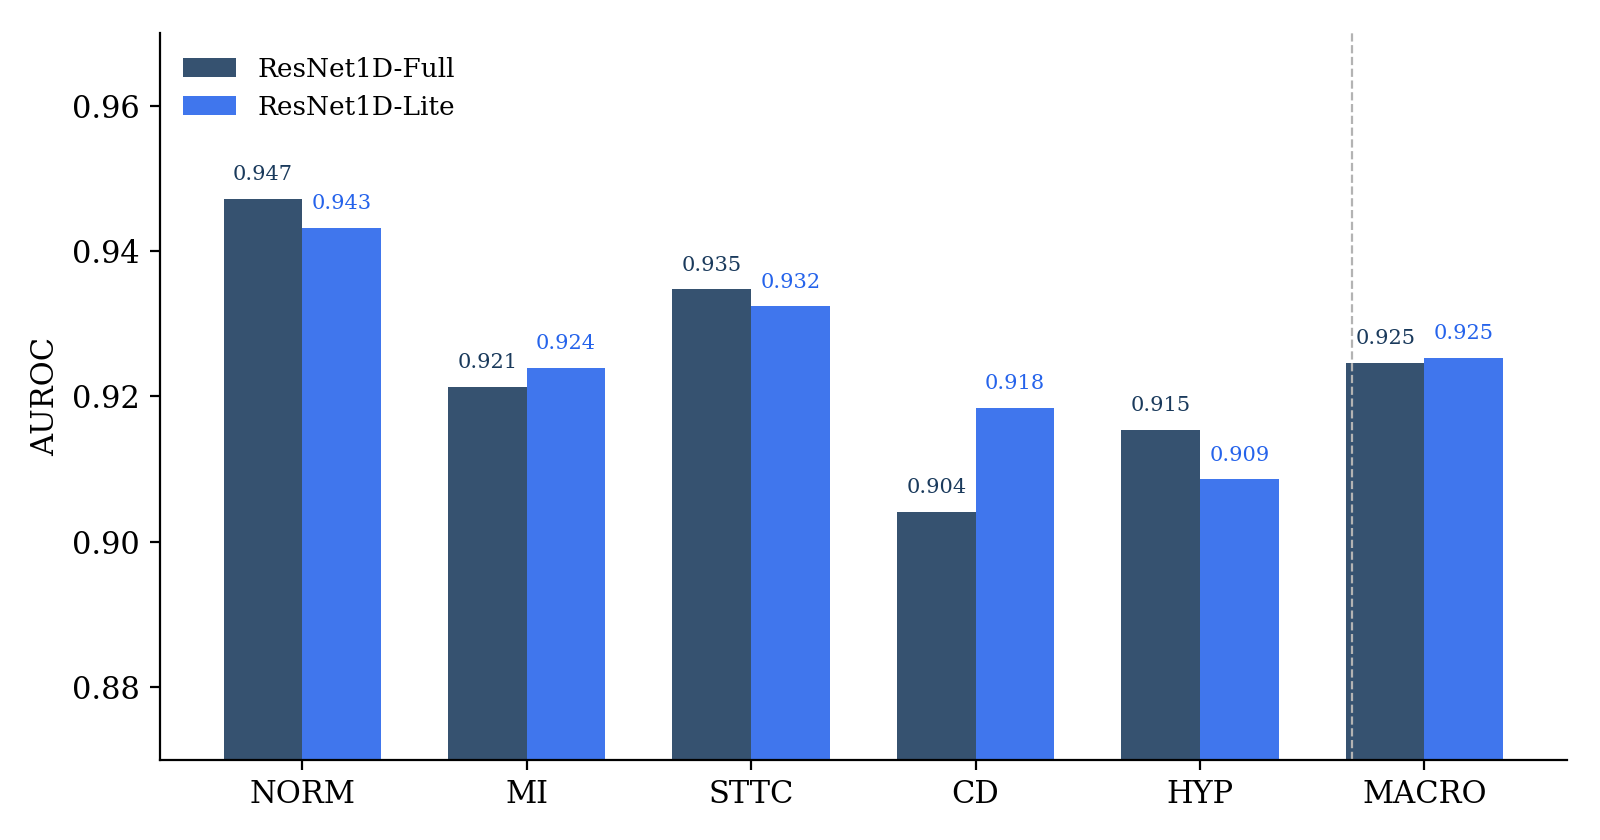
\includegraphics[width=0.88\textwidth]{fig_per_class_auroc.png}
\caption{Per-class and macro AUROC on the PTB-XL test set.
The dashed vertical line separates individual classes from the
macro average. ResNet1D-Lite matches or exceeds ResNet1D-Full
on MI and CD; differences elsewhere are $\leq 0.007$.}
\label{fig:auroc}
\end{figure}

\subsection{Training dynamics and generalisation}
Figure~\ref{fig:curves} shows validation AUROC and training loss over
40 epochs. Both models peak at epoch 17 with nearly identical validation
AUROC (0.9288 for Full, 0.9286 for Lite), then diverge: ResNet1D-Full
continues to drive training loss towards 0.059 and suffers a validation
AUROC decay of 0.0181 by epoch 40. ResNet1D-Lite plateaus at a higher
training loss (0.186) and its validation decay is only 0.0103---roughly
half of the larger model---indicating that capacity reduction acts as
implicit regularisation. The test-set advantage of ResNet1D-Lite is
consistent with this: despite a nominally identical best validation
checkpoint, the smaller model extracts more reusable representations
rather than memorising training-set specifics.

\begin{figure}[h]
\centering
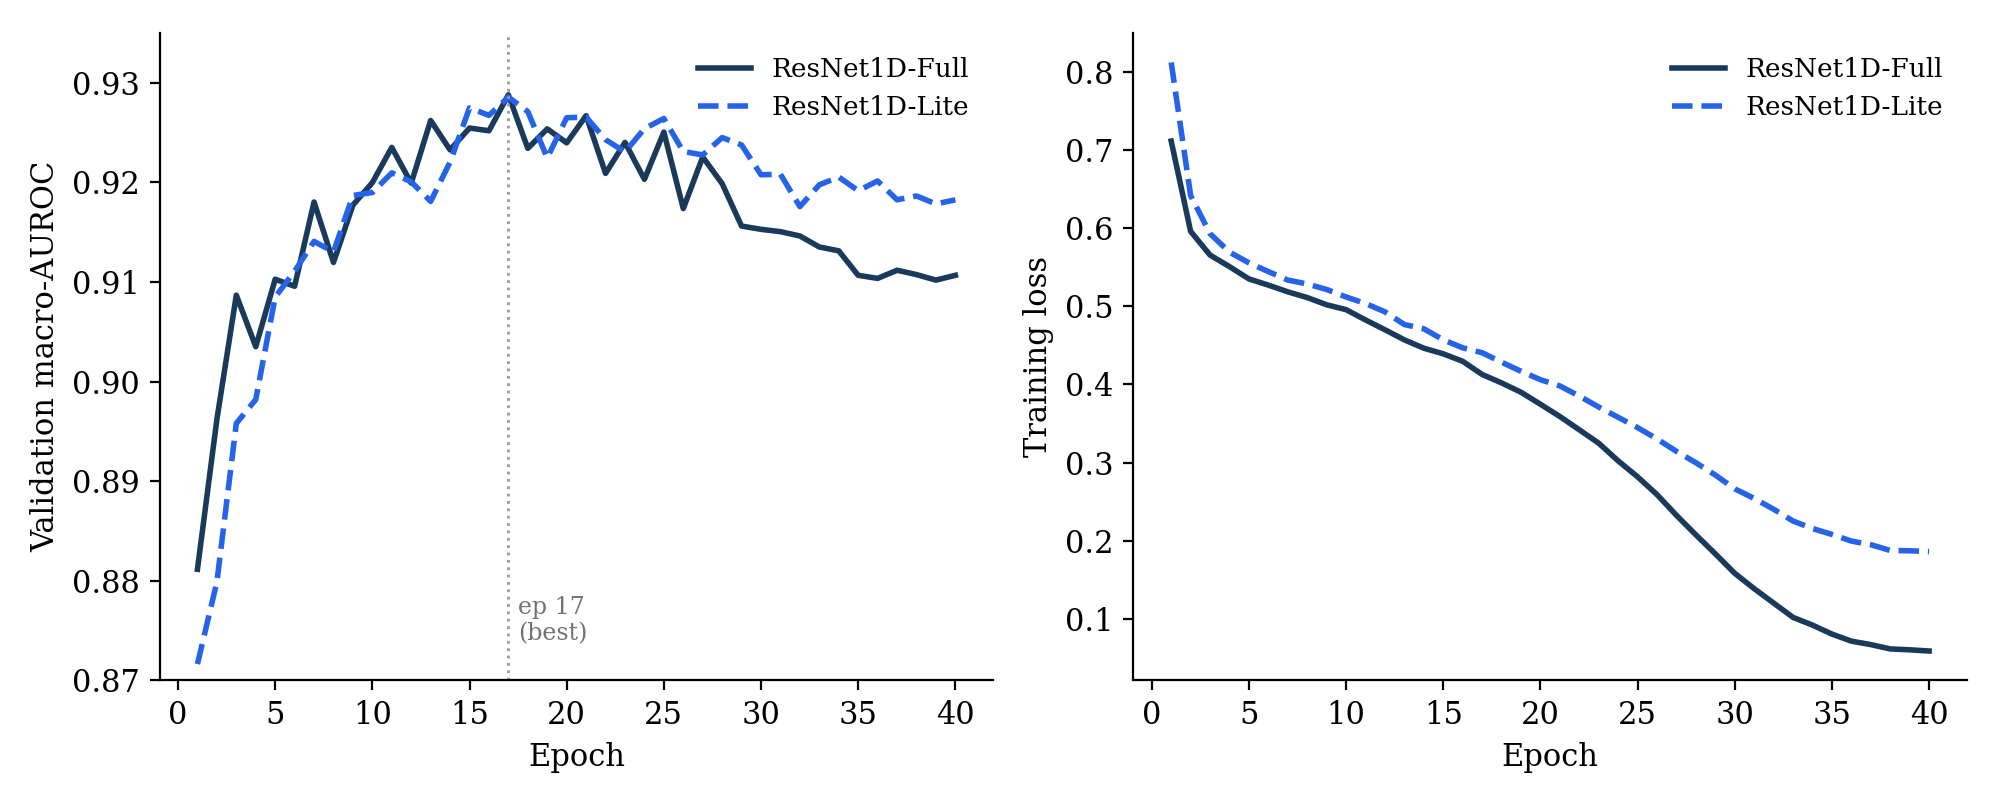
\includegraphics[width=0.92\textwidth]{fig_training_curves.png}
\caption{Validation macro-AUROC (\textit{left}) and training loss
(\textit{right}) over 40 epochs. Both models peak at epoch 17
(dotted vertical line). ResNet1D-Full overfits more severely in later
epochs, evidenced by a steeper loss decline without a corresponding
validation improvement.}
\label{fig:curves}
\end{figure}

\subsection{Comparison to published baselines}
Our macro AUROC values (0.9246--0.9253) are comparable to results
reported for convolutional architectures in the Strodthoff et
al.~\cite{strodthoff2021} PTB-XL benchmark. We note that exact
comparison is complicated by minor dataset versioning differences
and by the fact that Strodthoff et al. report confidence intervals
via bootstrapping; our results fall within the range of competitive
single-model performance reported there. The key distinction of our
work is not advancing the AUROC frontier but demonstrating that the
frontier is accessible to a model $8.65\times$ smaller.

\section{Discussion}
The primary finding is that ResNet1D-Lite, at 1.0\,M parameters and
4\,MB of storage, matches ResNet1D-Full (8.6\,M parameters, 34.5\,MB)
on the PTB-XL diagnostic superclass task and slightly surpasses it
on the macro average. This result has direct implications for deployment.
A 4\,MB model can be stored and loaded on a low-end Android tablet;
it can be transmitted over a slow or metered connection; and its inference
time on CPU is proportionally lower. For a Raspberry Pi 4 or comparable
single-board computer---the kind of hardware that might serve as a
point-of-care ECG workstation in a rural African clinic---the difference
between a 35\,MB and a 4\,MB model translates directly to latency and
battery life.

The CD superclass result (+0.014 for Lite) is the largest per-class
gap and merits attention. Conduction disturbances are morphologically
diverse and may be more susceptible to overfitting in a high-capacity
model than conditions with more stereotyped waveform signatures
(e.g.~NORM or HYP). The smaller model's superior CD performance
is consistent with the generalisation analysis: lower training-set
memorisation leaves the model better calibrated to the statistical
structure of CD patterns in unseen data.

\section{Limitations}
The evaluation is restricted to a single dataset and a single architecture
family; performance on other cohorts or with alternative model designs
may differ. We do not measure inference time on target hardware (CPU,
embedded device), which would strengthen the deployment argument. Model
calibration (reliability diagrams) is not assessed. Both models were
trained from random initialisation; pre-training on a larger corpus or
self-supervised pre-training may alter the efficiency--accuracy trade-off.

\section{Conclusion}
We trained two 1D residual networks of markedly different sizes on the
PTB-XL diagnostic superclass task. ResNet1D-Lite, with 1.0\,M parameters
and a 4\,MB footprint, matches and marginally exceeds the 8.6\,M-parameter
ResNet1D-Full on macro AUROC (0.9253 vs 0.9246) while generalising more
robustly in late training. The result supports the practical deployment
of compact ECG classification models in resource-constrained clinical
settings, where model size and inference cost are binding constraints.
Code and training notebook are publicly available.

\section*{Reproducibility}
All experiments were run on the PTB-XL dataset using the standard
recommended split. The full training notebook, including data loading,
model definitions, and evaluation code, is released at
\url{https://github.com/craigouma}.

\begin{thebibliography}{9}

\bibitem{wagner2020ptbxl}
P.~Wagner, N.~Strodthoff, R.-D.~Bousseljot, D.~Kreiseler, F.~I.~Lunze,
W.~Samek, and T.~Schaeffter,
``PTB-XL, a large publicly available electrocardiography dataset,''
\emph{Scientific Data}, vol.~7, no.~1, p.~154, 2020.


\bibitem{strodthoff2021}
N.~Strodthoff, P.~Wagner, T.~Schaeffter, and W.~Samek,
``Deep learning for ECG analysis: Benchmarks and insights from PTB-XL,''
\emph{IEEE Journal of Biomedical and Health Informatics}, vol.~25, no.~5,
pp.~1519--1528, 2021.


\bibitem{hannun2019}
A.~Y.~Hannun, P.~Rajpurkar, M.~Haghpanahi, G.~H.~Tison, C.~Bourn,
M.~P.~Turakhia, and A.~Y.~Ng,
``Cardiologist-level arrhythmia detection and classification in ambulatory
electrocardiograms using a deep neural network,''
\emph{Nature Medicine}, vol.~25, no.~1, pp.~65--69, 2019.

\bibitem{he2016}
K.~He, X.~Zhang, S.~Ren, and J.~Sun,
``Deep residual learning for image recognition,''
in \emph{Proc. IEEE Conf. Computer Vision and Pattern Recognition (CVPR)},
pp.~770--778, 2016.

\bibitem{loshchilov2019}
I.~Loshchilov and F.~Hutter,
``Decoupled weight decay regularization,''
in \emph{Proc. International Conference on Learning Representations (ICLR)},
2019.

\bibitem{pytorch}
A.~Paszke, S.~Gross, F.~Massa, A.~Lerer \emph{et al.},
``PyTorch: An imperative style, high-performance deep learning library,''
in \emph{Advances in Neural Information Processing Systems (NeurIPS)},
vol.~32, 2019.

\bibitem{who2021}
World Health Organization,
``Global health workforce statistics,''
\emph{WHO Data Repository}, 2021.
\url{https://www.who.int/data/gho/data/themes/topics/health-workforce}

\end{thebibliography}

\end{document}
